In this section, we explain in detail our encoding of the UC security definition into Nomos-UC.
Recall from Section~\ref{sec:background} that the UC security definition $\F_1 \xrightarrow{\pi} \F_2$ says we can realize some desired application $\F_2$ with a protocol $\pi$ that uses $\F_1$.
More generally, we define UC realization in terms of an indistinguishability relation between two experiments: the real-world featuring the execution of $\pi$ with $\F_1$, and an ideal-world execution of $\F_2$ with an ideal protocol $\idealP$ that relays inputs/outputs directly to/from $\F_2$.%
\footnote{This ideal protocol $\idealP$ is also the identity, since we can easily show $\F \xrightarrow{\idealP} \F$ for any functionality $\F$.}
Below, we introduce how the UC experiment is defined in NomosUC, and then provide a composition operator $\circ$ for protocols and simulators that satisfies Theorem~\ref{thm:singlecomp}.

\subsection{The UC Experiment}
%The UC experiment is an execution of protocol parties and an ideal functionality, reacting to input by an adversary \A or the environment \Z.
The type definition of \inline{execUC} is straightforward \todo{once we have clarity on the intro and type system section length we can include the typedef of here, it's not very interesting imo}. 
It is parameterized by at least one virtual token type to allow for sandboxing of other processes (usually by the adversary or environment) and message types specified by the protocol in question. 
Its only functional parameters are the security parameter $k$ and a random bit string $r$. 
It offers the following type \m{execout}:
{\centering
\parbox{0cm}{
\begin{tabbing} 
 $\m{execout}[a] = \textcolor{red}{\getpot^n} \echoice{\mb{exec}: $\=$ \ichoice{ \mb{out}: Bit \product 1}}$ 
 \end{tabbing}}
}
The spawning procss for \m{execUC} must provide it some number of tokens $n$ before the experiment starts. 
NomosUC forces us to be explicit in the polynomials used when checking a polynomial bound in the type system, and, as long as \m{execUC} is provided a number of tokens $n \in poly(k)$, Theorems~\ref{thm:global_ppt} and \ref{thm:preservation} guarantee that the experiment terminates in $poly(k)$. Therefore, we can conclude that every process in the experiment is also running time polynomial in $k$.  

%\begin{figure*}
%\begin{lstlisting}[basicstyle=\footnotesize\BeraMonottFamily, mathescape, frame=single]
%$\nproc$ execUC[K][p2f,f2p][z2p,p2z][a2p,p2a][f2a,a2f]{p2fn,f2pn}{z2pn,p2zn}{a2pn,p2an}{f2an,a2fn}{n}: 
%  (k: Int), (rng: [Bit]) |- ($\$$d: execout)
%\end{lstlisting}
%\caption{Type definition for \m{execUC} with no virtual tokens.}
%\label{fig:execuc}
%\end{figure*}

The type parameters of \m{execUC} are parameters to the channels spawned between the main processes.
For example, the channels between \Z and \A are instantiated as
\begin{lstlisting}[basicstyle=\footnotesize\BeraMonottFamily, mathescape]
#z_to_a $\leftarrow$ channel_init[$\tp{K}$][$\tp{z2a}$]{$\tp{z2an}$}
#a_to_z $\leftarrow$ channel_init[$\tp{K}$][$\tp{a2z}$]{$\tp{a2zn}$}
\end{lstlisting}
where its import parameters $\tp{z2an}$ and $\tp{a2zn}$ (the import amount) are also type parameters of \inline{execUC}.
%When processes are spawned, their shell codes correctly connect the channel endpoints internally.
We point out that process definitions for \Z, \A, \F, and $\Pi$ are not passed as parameters to \inline{execUC} because NomosUC currently doesn't support passing them as parameters.

The environment \Z is the first main processes and offers the type \m{EtoZ} (below) to \m{execUC}.
\Z sends an \mb{init} message with the list of corrupt parties and an SID (a user-defined type).
On \mb{start} by \m{execUC} along with $n$ import tokens, \Z begins with the execution, and it concludes with a output \mb{Bit} to \m{execUC}.
{\centering
\parbox{0cm}{
\begin{tabbing}
 $\m{EtoZ}[a] = \textcolor{red}{\getpot^n} \ichoice{\mb{init}: $\=$ SID[a] \arrow [PID] \arrow$ \\
\>$\echoice{\mb{start} \arrow \ichoice{\mb{out}: Bit \arrow 1}}}$
 \end{tabbing}}
}
The output bit, it's guess of which world it is in, forms the basis for the definition of indistinguishability.  	

%\begin{figure*}[t]
%\begin{lstlisting}[basicstyle=\scriptsize\BeraMonottFamily, frame=single, mathescape, caption={The process definition of the \msf{execUC} function.}]
%$\Stype$ Bit{n} = <{n}| &{ exec: +{out : Bit $\rightarrow$ 1}} ;
%
%$\tb{proc}$ execUC[$\tp{K}$][$\tp{K1}$][$\tp{sid}$][$\tp{p2f,f2p}$][$\tp{z2p,p2z}$][$\tp{a2p,p2a}$][$\tp{a2f,f2a}$]{$\tp{p2fn,f2pn}$}{$\tp{p2zn,z2pn}$}{$\tp{a2pn,p2an}$}{$\tp{a2fn,f2an}$} :
%  (k: $\tgr{int}$), (r: [Bit]) |- ($\$$d: Bit)
%\end{lstlisting}
%\label{lst:execuc}
%\end{figure*}

\subsection{The \partywrapper}
\begin{figure}
	\centering
	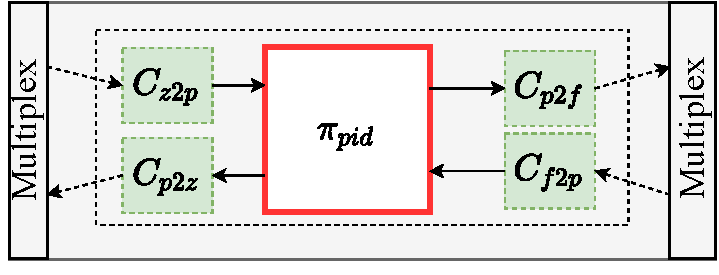
\includegraphics[scale=0.5]{figures/singleshellmultiplex.pdf}
	\caption{This is the \partywrapper that routes messages to the correct internally runnint protocol party. This figure shows how one protoco party (dotted box) is instantiated within it. The party $\pi_{pid}$ is shell code akin to Figure~\ref{fig:newpandq}.}%\snote{Updated caption to say it's multiplexer with one instance. The reason I don't want to include another instance is that I couldn't figure out a way to add it and expand the diagram horizontally. It will leave so much white space on the sides if I add a new party and will take up much more vertical space which we need to cut down on anyway.}}
	\label{fig:singlemultiplex}
	\vspace{-3mm}
\end{figure}
The \partywrapper spawns protocol parties, runs them in a sandbox, and routes messages to/from them and \Z, \F, and \A.
As a result of using channels, NomosUC needs the \partywrapper to handle the dynamic creation of parties: spawning processes, creating the channels they require, and connecting them to the rest of the experiment.

We achieve this in two ways: by our providerless channels construction and by sandboxing protocol parties within the \partywrapper.
Instead of parties directly connected to \F and \Z through a providerless channel, the \partywrapper runs them virtually, internally, but presents a view to them as if they are directly connected to \F and \Z. 
In fact, the \partywrapper is connected by single channels to \F, \Z, and \A, and it routes communication to/from the appropriate protocol party. 
In Figure~\ref{fig:singlemultiplex}, we see an instance of a protocol party within the \partywrapper that is connected to processes offering it linear channels for communication with \Z and \F. 
This is only the part of the providerless channel connected to the party, whereas the other end is handled by the \partywrapper.

Like the providerless channels, which rely on some code generation, the \partywrapper also relies on the code generation to create processes which can convert messages from the single providerless channel between, say, \partywrapper and \F  and the individual linear channels offered to each protocol arty.
Typically, such protocol-specific communication constructs are written by users, as is the case with the addressing scheme in EasyUC~\ref{easyuc}, but in NomosUC the processes themselves are so trivial (akin to a function application on messages) that they can be generated easily.

One tradeoff with the \partywrapper design is that the import sent to it by \F, \Z, and \A must be constant as they each communicate with it over a single providerless channel.  
In the sandbox, however, the protocol parties receive virtual import tokens according to the varying amounts specified by the session types.
We don't see this as a downside of the approach as tight runtime constraints or reasoning is not an intended goal of NomosUC or the UC framework.

\paragraph{Functionalities}
Like the \partywrapper, we also treat functionalities are being wrapped by code that handles communication with other processes. The wrapper around a functionality creates the same dummy processes as in the \partywrapper with the desired session type.
In the \Fcom example, the \partywrapper creates dummy processes that offer the \m{sender} and \m{receiver} session types to the sender and receiver, and the functionality's wrapper does the same for \Fcom. 

\paragraph{Functionalities}
Like the \partywrapper, we also treat functionalities are being wrapped by code that handles communication with other processes. The wrapper around a functionality creates the same dummy processes as in the \partywrapper with the desired session type.
In the \Fcom example, the \partywrapper creates dummy processes that offer the \m{sender} and \m{receiver} session types to the sender and receiver, and the functionality's wrapper does the same for \Fcom. 

%For the remainder of this work we denote and individual protocol party as $\pi$ or $\pi_i$, and a protocol as a whole run inside the \partywrapper as $\m{MX}(\Pi)$ or $\m{MX}(\pi)$.


\subsection{Emulation}
The central security definition in UC is indistinguishability between the real and ideal world experiments.
In NomosUC, we define the term \textit{well-matched} to mean the configuration resulting from a PPT term $e$ connected to another term $e'$ in well-typed, and we denote it as: $e \leftrightarrow e'$.
The term allows us to quantify statements over only adversaries and environments whose types match the protocol/functionality in question when reasoning about emulation. 

We define indistinguishability in terms of te ensemble of distributions of the output bit of the partial term $\m{execUC}\ \pi\ \F$ over all possible bitstrings and security parameters using the standard way of statistical distribution.  

%We define the output bit of the partial term of \inline{execUC}, for a specific $\pi$ and \F, as an ensemble of distributions over all possible random bitstrings and security parameters.
%Emulation, then, is about the ensembles created by two UC executions being computationally indistinguishable from each other.
%We define indistinuishability between ensembles in a standard way using \textit{statistical distance}: $\mathcal{D}_{1,k} sim \mathcal{D}_{2,k}$ if their statistical distance is at most $negl{k}, \forall k$.
%\begin{definition}[Indistinguishability]\label{def:distance}
%Two ensembles $\mathcal{D}_{1,k}, \mathcal{D}_{2,k}$ are indistinguishable, $\mathcal{D}_{1,k} \sim \mathcal{D}_{2,k}$, if their statistical distance is at most $negl(k), \forall k$.
%\end{definition}

UC emulation combines the UC execution with indistinguishability resulting in the following NomosUC emulation definition.
\begin{definition}[Emulation]\label{def:emulation}
If two protocols $(\pi, \F_1)$, $(\phi, \F_2)$, which we refer to only by \PI and $\phi$, emulated each other, then $\forall \A$ well-matched with \PI, there must $\exists \Sim$ well-matched with $\phi$ s.t. $\forall \Z$ : $\msf{execUC}(\pi, \F_1, \Z, \A)$ $\approx$ $\msf{execUC}(\phi, \F_2, \Z, \Sim)$:

\begin{mathpar}
	\footnotesize
	\inferrule*[right=emulate]
	{
		\pi : \Delta_1'[\Tokentypes][\mathrm{T}_{\pi}] \semi \phi : \Delta_2'[\Tokentypes][\mathrm{T}_{\phi}] \semi \\
		\forall \A \ | \ \Delta_4[\Tokentypes][\mathrm{T}_{\A}] \vdash \A :: \Delta_3', \ \langle \A \leftrightarrow \pi \rangle \\
		\Rightarrow \exists \ (\Delta_3[\Tokentypes][\mathrm{T}_{\Sim}] \vdash \Sim_\A :: \Delta_3') \ | \ \langle \Sim_\A \leftrightarrow \phi \rangle \\
		\Rightarrow \forall \Z  \; \msf{execUC} \ \pi\ \F_1\ \Z\ \A \approx\ \msf{execUC} \ \phi\ \F_2\ \Z\ \Sim_\A
	}
	{
		% EMULATION DEFINITION
		\lambda \A \, . \, \Sim_\A \vdash (\pi, \F_1) \sim (\phi, \F_2)
	}
\end{mathpar}
\end{definition}

An important validation of our approach is the the Dummy Lemma~\ref{thm:dummythicclemma} which shows that a simulator, \DS, for the dummy adversary satisfies the emulation definition for all adversaries \A. 
\begin{theorem}[Dummy Lemma]\label{thm:dummythicclemma}
If \ $\exists \DS$ s.t. $ \DA, \DS \vdash \F_2 \xrightarrow{\pi} \F_1$ then $\forall \A \ \exists \Sim_\A$ s.t. $\Sim_{\A} \vdash  \F_2 \xrightarrow{\pi} \F_1)$ 
\end{theorem}
The proof of the Lemma is in the form of a simulator that combines the real world adversary and the dummy simulator in a straightforward way (in Appendix~\ref{sec:dummy}. Though a simple construction it illustrates the simplicity of our sandboxing and allows us to work only with dummy simulators from now on.

\subsection{Single Composition}
In this section we present a composition operator for protocols that completes the single composition theorem, Theorem~\ref{thm:singlecomp}.
The composition operator allows replacement of a single instance of a functioality with a protocol realizing it, and, potentially, any functionality that protocol uses.

In NomosUC, composition of protocols occurs in the \partywrapper where output from $\rho_i$ to $\F_2$ is given as input to $(\pi, \F_1)$. $\pi$ runs in the \partywrapper and $\F_1$ is the hybrid functionality. 
The operator connects parties of $\rho$ and $\pi$ through providerless channels where $\rho$ gives input to $\pi$. 
Like \m{execUC} (whose code can be seen in the Appendix), the operator spawns a providerless channel to intermediate communication between the two protocols, spawns their wrapper processes, and returns:

\begin{lstlisting}[basicstyle=\footnotesize\BeraMonottFamily, mathescape, frame=single]
#rho2pi $\leftarrow$ channel_init[K][rho2f]{rho2fn} ;
#pi2rho $\leftarrow$ channel_init[K][f2eho]{f2rhon} ;

$\$$r $\leftarrow$ rho <- k rng sid pid #z2p #p2z #rho2pi #pi2rho; 
$\$$p $\leftarrow$ pi <- k rng sid pid #rho2pi #pi2rho #p2f #f2p;
\end{lstlisting}

Recall that every protocol and functionality comes with generated processes which handle communication as part of the providerless channels as depicted in Figure~\ref{fig:newpandq}.
In the code snippet above, this means that \inline{rho} and \inline{pi} are wrappers that encapsulate the actual protocol and the generated processes, and passing the channel endpoints to the shell connects them correctly. 

%The processes \inline{rho} and \inline{pi} are actually wrapped processes like the one depicted in Figures~\ref{fig:newpandq} and \ref{fig:singlemultiplex}.
%The challenge in creating a generic composition operator is managing protocol and type-specific providerless channels.  
%As we stated previously, the \partywrapper and protocol channels rely on some code generation in order to make use of expressive session types, and the composition operator is now different.
%In our construction above, 

%The generic composition operator of NomosUC connects the shells of parties $\rho_i$ and $\pi_i$ through providerless channels. 
%As mentioned earlier, for functionalities/protocols that don't need to split communication over two channels, the coposition operator can be trivialized by directly connected the channel offered by $\rho_i$ as the input channel of $\pi_i$.
%The type system here guarantees that our composition gives $\pi_i$ an appropriate amount of import and tha the resulting protocol is also polynomially bound. 

Part of the security proof of security under composition is providing a simulator that ensures emulation.
For this we can define simulator compostion operator that connects the simulators \SIM{\rho} and \SIM{\pi} in the natural way: pipe output from \SIM{\pi} to \SIM{\rho} and vice versa.
The providerless channel abstraction makes the construction simple to realize and involves only simple function application to messages.
%Inputs to the adversary are intended for $\F_1$ or dummy parties of $\F_1$ and are handled by \SIM{\pi}. Outputs from \SIM{\pi} are intended for $\F_2$ and dummy parties of $\F_2$ is simulated by \SIM{\rho}.

\subsection{UC Composition}

\begin{theorem}[Composition]\label{thm:composition}
\begin{mathpar}
\inferrule*[right=compose]
{
	%(\pi, !\F_1) \sim (\idealP, F_2) \semi (\rho, !\F_2) \sim (\idealP, \F_3) \\ 
	!\F_1 \xrightarrow{\pi} \F_2 \semi !\F_2 \xrightarrow{\rho} \F_3 \\
	%\Rightarrow \exists \Sim(\A) \vdash (\rho^{!\F_2 \rightarrow (!\pi \, \circ \, \msf{squash})}, !\F_1) \sim (\idealP, \F_3)
}
{
	!\F_1 \xrightarrow{\rho \, \circ !\pi \circ \, \msf{squash}} \F_3
	%(\rho \, \circ \, !\pi \circ \msf{squash}, !\F_1) \sim (\idealP, \F_3)
}
\end{mathpar}
\end{theorem}

Full composition in the UC framework extends beyond the simpler composition in Theorem~\ref{thm:singlecomp} allowing replacement of only one instance of a functionality with a protocol that realizes it.
Instead, UC composition allows for replacement of any number of instances of a functionality with instances of the realizing protocol.
Theorem~\ref{thm:composition} illustrates the full composition theorem using our arrow notation, and highlights a theorem that we must prove before we can achieve full composition.
%We rely on two sub-theorems that make use of the multisession extension: Theorem~\ref{thm:squash} and Theorem~\ref{thm:functor}.
We rely on a sub-theorem that makes use of the multisession extension: Theorem~\ref{thm:functor}.
\begin{theorem}[Multisession Composition]\label{thm:functor}
	\begin{mathpar}
		\inferrule*[right=MultiComp]
		{
			\F_1 \xrightarrow{\pi} \F_2
		}
		{
			!\F_1 \xrightarrow{!\pi} !\F_2
		}
	\end{mathpar}
\end{theorem}
The detailed description of this extension and its security proof can be found in the Appendix. At a high level is shows that security holds when protocols/functionalities are arbitrary replicated and run concurrently.
We also prove an adjacent Theorem~\ref{thm:squash}, in the appendix, which allows squashing a doubly-applies multi-session extension to a single application of it with a \msf{squash} protocol ($!!\F \xrightarrow{\msf{squash}} !\F)$.

Defining these extensions, theorem and their simulators in NomosUC allows us to conclude that NomosUC captures the full, generlized UC composition theorem with the following argument. 

\begin{proof}
By Theorem~\ref{thm:singlecomp} we have that $\F_1 \xrightarrow{\pi} \F_2$. If we combine this result with Theorem~\ref{thm:functor} we can conclude that $!!\F_1 \xrightarrow{\rho \circ !\pi} !\F_3$. 
Finally we can squash one $!$ operator with Theorem~\ref{thm:squash} (in Appendix~\ref{app:ms}) to get $!\F_1 \xrightarrow{\rho \circ !\pi \circ \m{squash}} \F_3$.
\end{proof}


